% \documentclass[article, oneside]{memoir}
\documentclass[oneside, 11pt]{article}

\usepackage[utf8]{inputenc}
\usepackage{graphicx}
\usepackage{natbib}
\usepackage{astrojournals}
\usepackage{booktabs}
\usepackage{url}
% \usepackage[osf]{newtxtext}
% \usepackage[libertine]{newtxmath}
% \usepackage{arev}
\usepackage[varg]{txfonts}

\title{No evidence for an optically thin circumstellar disk in Orion\thanks{Not submitted anywhere, yet.}}
\author{William J. Henney\thanks{
    Centro de Radioastronomía y Astrofísica, 
    Universidad Nacional Autónoma de México, Mexico.  
  }\\
  \protect\footnotesize\url{w.henney@crya.unam.mx}
  }
\date{Draft version 1: 2013 August 26}

\begin{document}
\maketitle

\begin{abstract}
  I present an analysis of archival \textit{HST} images of  the Orion Nebula silhouette disk 218-354, obtained at multiple epochs and with two different cameras.   By comparing exposures taken with different telescope orientations, it is possible to correct for some instrumental artifacts in the images.   In agreement with previous \textit{HST} measurements, I find that the inner \(0.4''\) (180~AU) portion of the disk is optically thick at 6563~\AA{}, the wavelength of  the H\(\alpha\) line.   This result contradicts a recent claim, based on adaptive optics observations, that the disk is optically thin at H\(\alpha\).
  % \citet{Follette:2013a} present adaptive optics observations of the Orion Nebula silhouette disk 218-354, and claim that the disk is optically thin in H\(\alpha\).  I point out that existing \textit{Hubble Space Telescope} observations with two different cameras demonstrate that this claim is false.  The inner \(0.4''\) (180~AU) portion of the disk appears to be totally opaque at the wavelength of H\(\alpha\), although a translucent outer portion extends out to about \(0.7''\) (300~AU).

% It's not a rebuttal -- it's a refutation. 
\end{abstract}

\clearpage
\section{\textit{HST} observations of 218-354}
\label{sec:hst}


\begin{table}
  \caption{HST imaging of the 218-354 disk}
  \label{tab:hst}
  \centering
  \smallskip
  \begin{tabular}{llll}\toprule
  Program & Year & PI & Camera/Detector \\ \midrule
  5085 & 1995 & C. R. O'Dell & WFPC2/WF \\
  8121 & 2000 & C. R. O'Dell & WFPC2/WF \\
  9825 & 2004 & J. Bally & ACS/WFC \\
  10246 & 2004/5 & M. Robberto & ACS/WFC + WFPC2/WF\\ \bottomrule
\end{tabular}
\end{table}

The circumstellar disk 218-354 has been imaged in H\(\alpha\) many times with the \textit{HST} between 1995 and 2005  \citep{McCaughrean:1996a, ODell:2001c, Bally:2006a, Ricci:2008a, Robberto:2013a}.   Details of the programs are given in Table~\ref{tab:hst}.  The cameras/detectors used were the Wide Field CCDs of the \textit{Wide Field and Planetary Camera 2} (WFPC2/WF, pixel size: \(0.1''\)) and the Wide Field Channel of the \textit{Advanced Camera for Surveys} (ACS/WFC, pixel size: \(0.05''\)).   

Four of the most recent images of 218-354 are shown in Figure~\ref{fig:hst-images}.   Technical details of the observations are given in the figure caption.   In all cases, the disk is clearly seen as an elliptical shadow that blocks the H\(\alpha\) emission from the ionized gas in the Orion Nebula, which lies behind it.   Earlier observations are shown in Fig.~1 of \citet{McCaughrean:1996a}. 

\begin{figure}
  \centering
  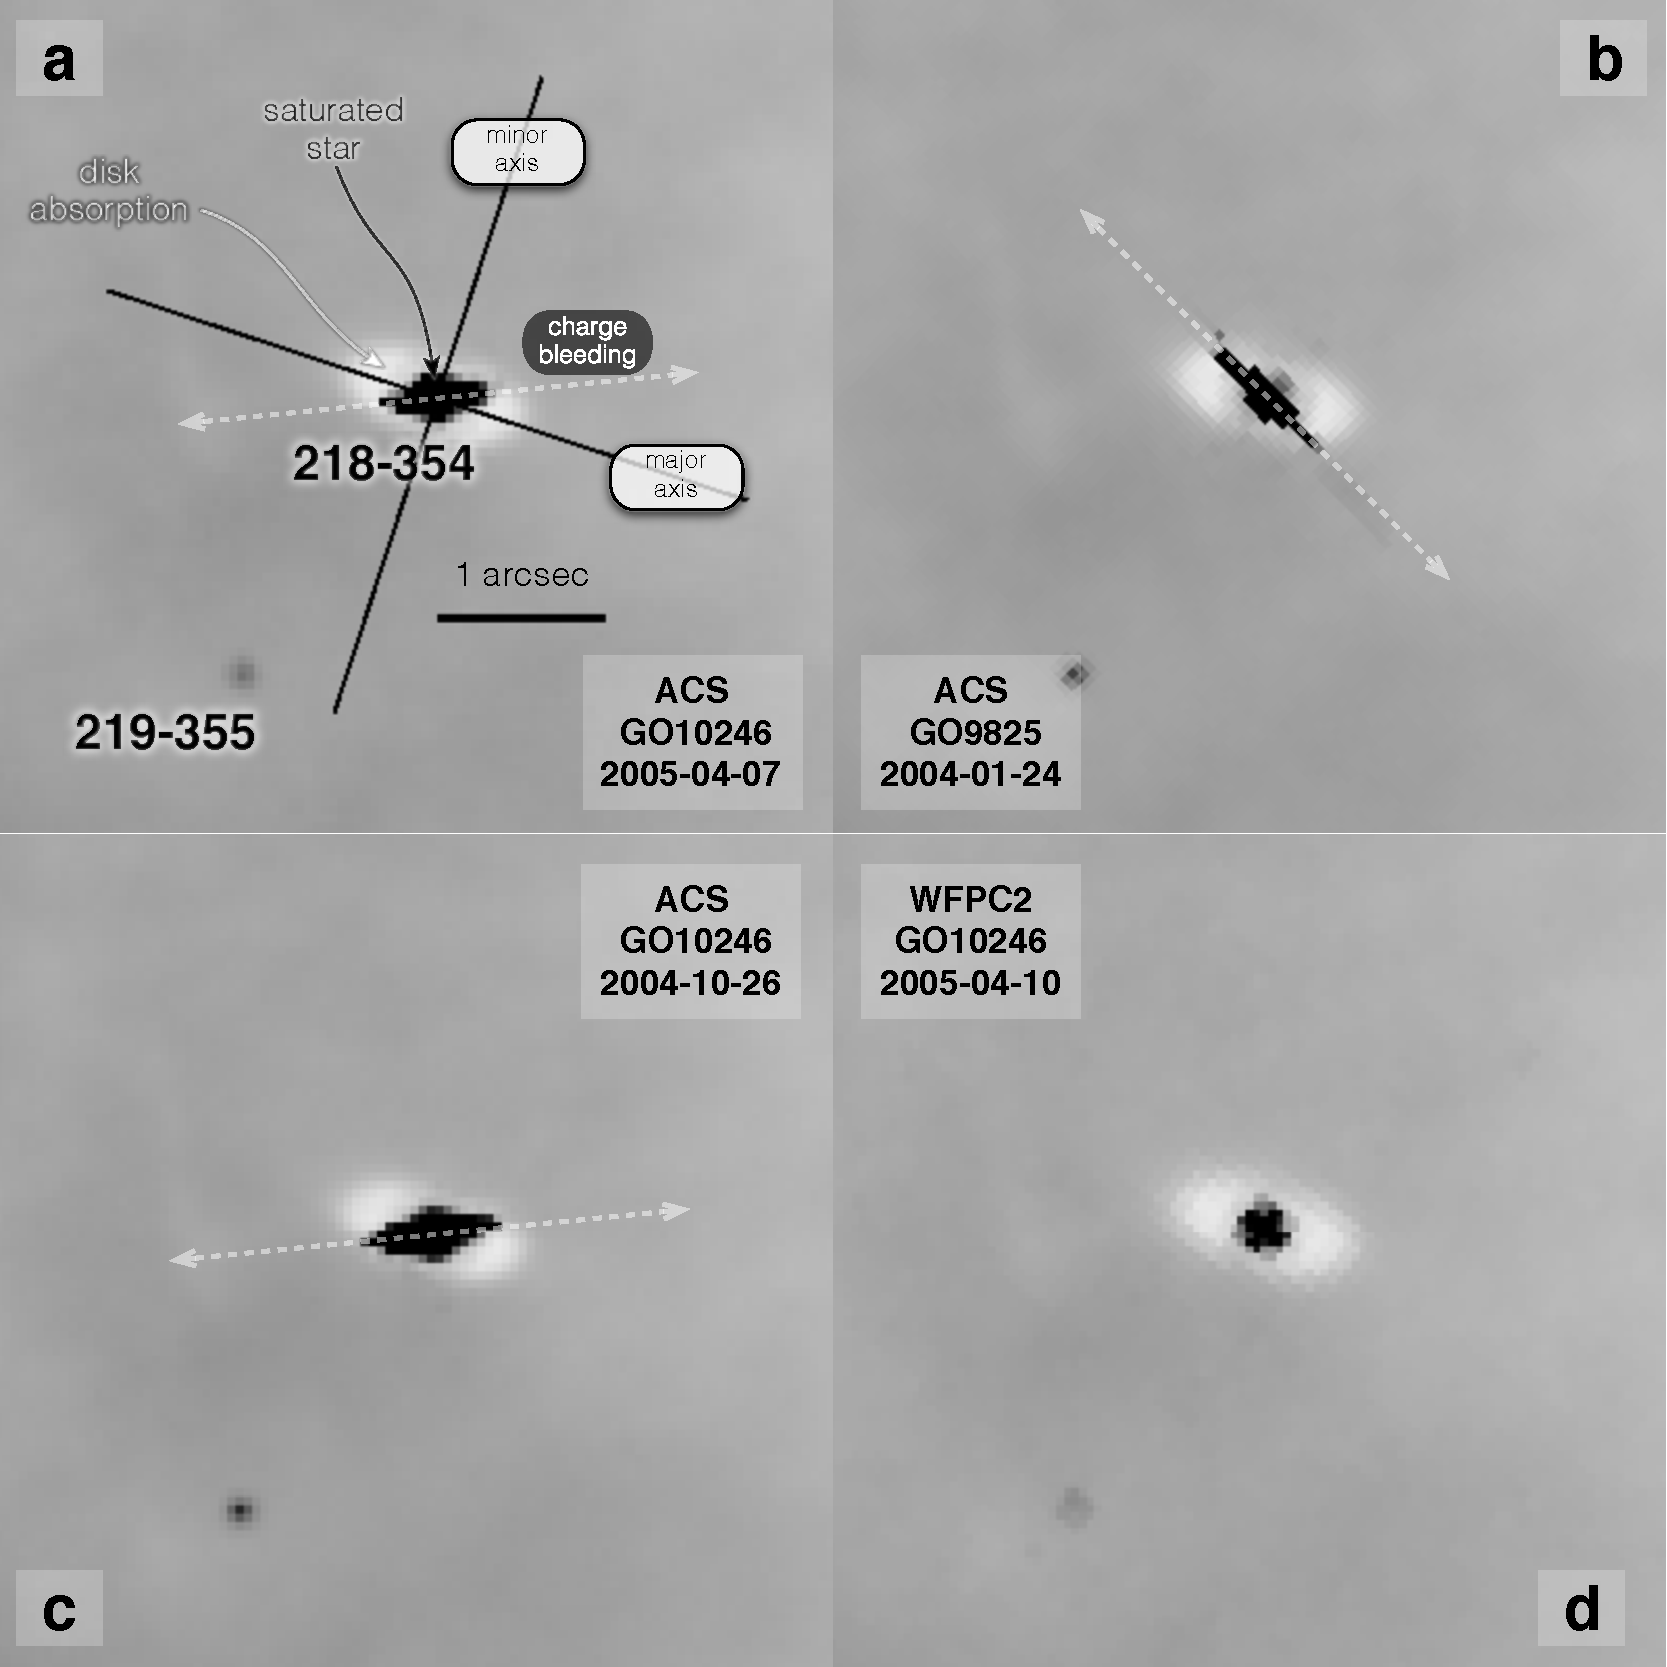
\includegraphics[width=\linewidth]{four-images-218-354}
  \caption[]{Negative images of the protoplanetary disk 218-254 obtained with the \textit{Hubble Space Telescope}, using different instruments and detector orientations.  (\textit{a})~ACS image from program GO10246, visit 0B \citep{Robberto:2013a}.  (\textit{b})~ACS image from program GO9825 \citep{Bally:2006a}.  (\textit{a})~ACS image from program GO10246, visit 55.  (\textit{a})~WFPC2 image from program GO10246, visit 39.   In all cases, orientation is north up, east left.   The GO9825 image (panel \textit{b}) had to be shifted by \(\simeq 1.2''\) to bring it into alignment with the GO10246 images, which are all tied to the 2MASS absolute astrometric reference frame.  All images are the result of multiple exposures that have been combined by the MultiDrizzle algorithm, which corrects for geometric distorsion and removes cosmic rays.  During this process, the WFPC2 image has been resampled from the native WFC pixel size of \(0.1''\) to the PC pixel size of \(0.045''\).  All data were downloaded from the \textit{Barbara A. Mikulski Archive for Space Telescopes} (MAST: \url{http://archive.stsci.edu}) during 2013 August 15 to 21.  }
  \label{fig:hst-images}
\end{figure}


The major axis diameter of the disk is \(\simeq 1''\), which allows it to be well resolved by \textit{HST} (the diffraction limit FWHM at 6563~\AA{} is \(\simeq 0.07''\), which is adequately sampled by the ACS pixels).  Despite this, only the outer regions of the disk can clearly be seen in absorption, due to the bright continuum emission from 218-354's central star, which dominates the central regions (\(< 0.2''\)).   This contamination is particularly serious in the case of the ACS images because the central star saturates the detector, leading to charge bleeding along the read-out direction of the CCD (indicated by arrows in Fig.~\ref{fig:hst-images}). 

\begin{figure}
  \centering
  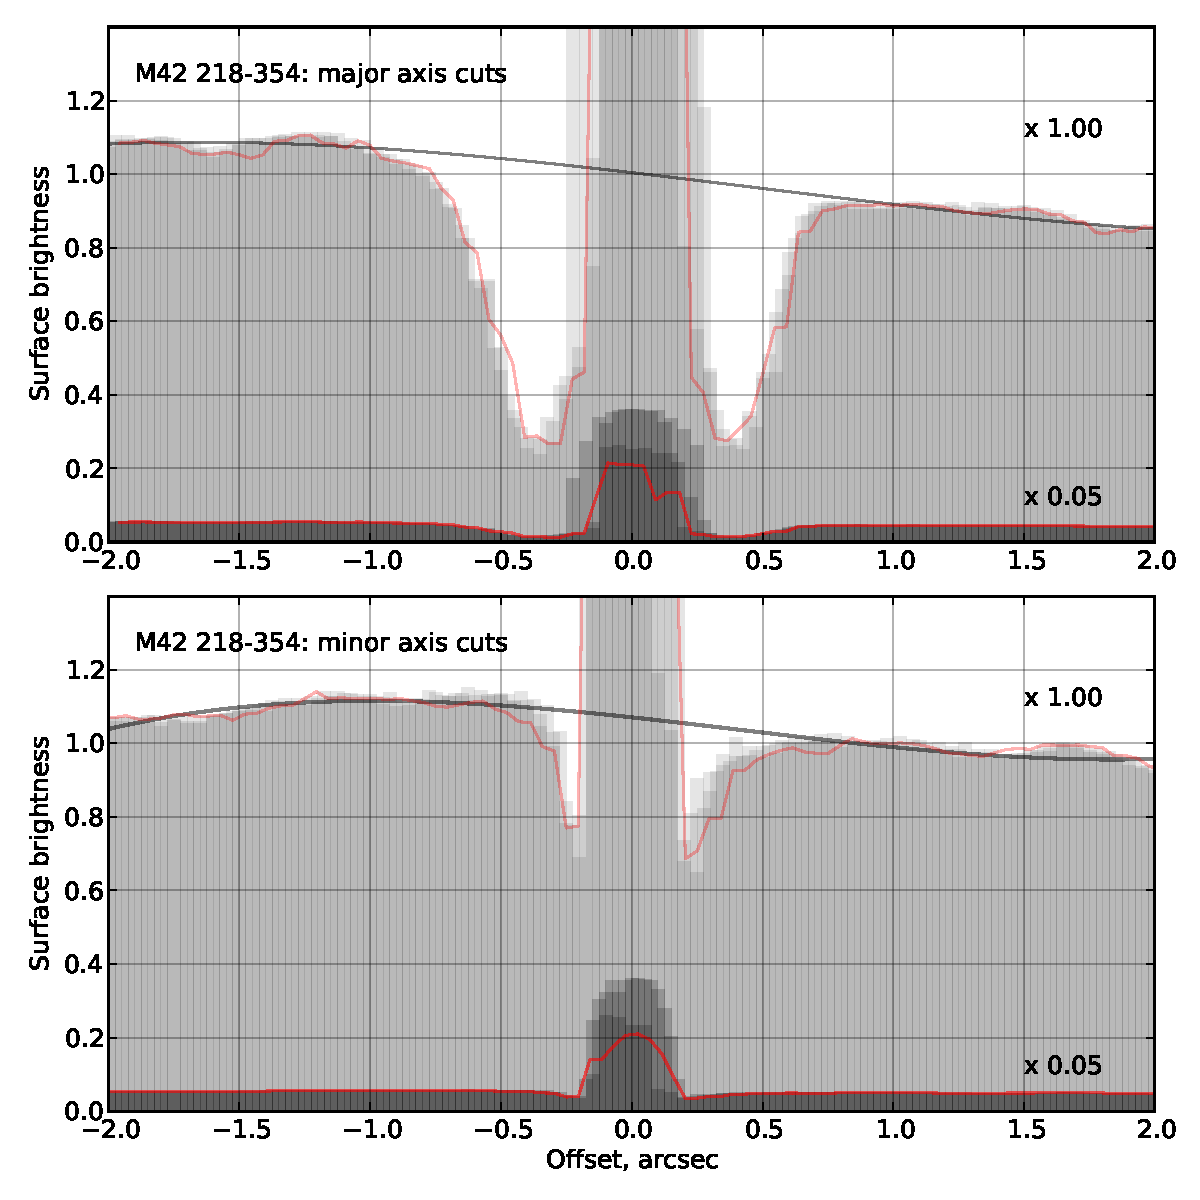
\includegraphics[width=\linewidth]{profiles-acs-218-354}
  \caption{Surface brightness profiles of the images shown in Fig.~\ref{fig:hst-images}, taken along the disk major axis (upper panel) and minor axis (lower panel).  
    The three ACS exposures are shown as overlapping translucent gray histograms, while the WFPC2 exposure is shown by red lines.
  The data are shown at two different brightness magnifications: the light gray histograms (\(\times 1.00\)) emphasize the disk absorption profile, while the dark gray histograms (\(\times 0.05\)) show the saturated emission profile of the central star.  
  The heavy gray lines show cubic polynomial fits to the nebular background emission. }
  \label{fig:hst-profiles}
\end{figure}

However, the availability of multiple images allows the effect of the saturated star to be easily tested, since the different telescope orientations mean that the CCD read-out axis corresponds to different position angles on the sky.   In Figure~\ref{fig:hst-profiles} I show brightness cuts (one pixel wide) along the major and minor axis for all four images.   It can be seen that there is excellent agreement in the profiles of the 3 ACS images (gray histograms) for positions \(> 0.35''\) from the central star.   The WFPC2 image is also consistent, except that the larger original pixel size and lower signal-noise degrade the effective resolution and tend to smooth out sharp gradients, especially noticeable along the minor axis.    Thus, the absorption profile of the disk can be reliably measured nearly all the way in to the apparent minimum in the brightness profile.   For positions closer to the star, the stellar PSF and charge bleeding start to dominate the profile (with a possible additional contribution from dust-scattered starlight in the inner disk).  In these regions, large variations are seen between the different ACS images due to the angular variation of the PSF, differing degrees of saturation, and the varying angle between the disk axis and the CCD read-out axis.   It is possible that careful PSF modelling and removal might allow the disk absorption profile to be recovered at smaller radii than \(0.35''\), but that is not necessary for the arguments of this paper.  

\section{Comparison with the claims of \citeauthor{Follette:2013a}}
\label{sec:comp}

\begin{figure}
  \centering
  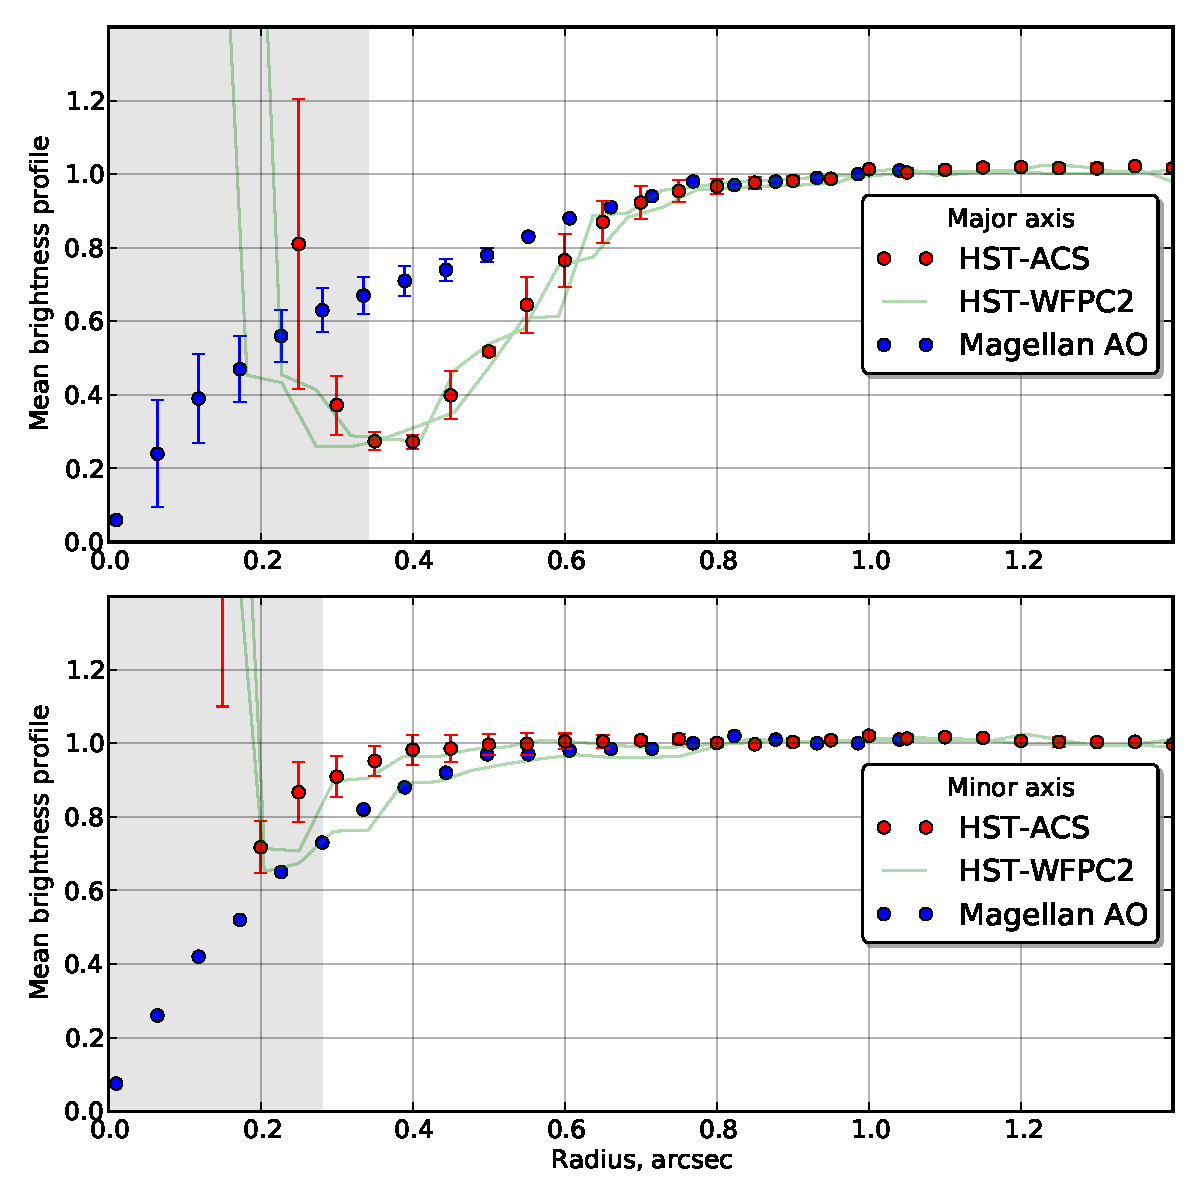
\includegraphics[width=\linewidth]{rprofiles-acs-218-354}
  \caption{Red points and error bars show average radial profiles along the major (upper panel) and minor (lower panel) axes of the 3 ACS images.  The profiles  are calculated on a regular grid with spacing 0.05 arcsec, using nearest-neighbor interpolation from the original images.    Profiles are normalized to the interpolated polynomial fit to the nebula background emission (see Fig.~\ref{fig:hst-profiles}).  The mean and standard deviation are calculated for each radial grid point (typically 6 image pixels contribute to each point).   Error bars are 1 sigma.   The gray shaded region indicates radii that are affected by the PSF and charge bleeding of the stellar profile.   Green lines show the lower-resolution WFPC2 profiles, with each semi-axis being shown separately.   Blue points and error bars show the reported radial profiles from Magellan AO observations \citep{Follette:2013a}, measured by eye from Fig.~2 in their published paper (no error bars are given for their minor axis profile).}

  \label{fig:compare}
\end{figure}

Figure~\ref{fig:compare} shows the average and standard deviation of the three ACS profiles from Figure~\ref{fig:hst-profiles} as a function of distance from the central star (red symbols and error bars).  Details of the averaging procedure are given in the figure caption.   The WFPC2 profiles are also shown (thin green lines), with each semi-axis plotted separately to illustrate the differing minor-axis profiles on the two sides of the disk.    The figure also shows (blue symbols and error bars) the equivalent results from Figure~2 of \citet{Follette:2013a}, which represent the radial profiles of continuum-subtracted H\(\alpha\) images with the \textit{Magellan Adaptive Optics} (MagAO) system, rebinned by a factor of 7 to pixels of \(0.055''\). 

It is apparent that there is a serious discrepancy between the \emph{HST} radial profiles and the reported MagAO profiles along the major axis.   Both sets of observations show that the outer extent of the disk extinction is at \(r \simeq 0.75''\), but the \emph{HST} profile swiftly falls to about 25\% of the background nebula brightness at \(r = 0.4''\), while the MagAO profile shows a very gradual decline with decreasing radius: at \(r = 0.4''\) it is still at \(> 70\%\) of the background brightness, and it only reaches the 25\% level very close to the star at \(r < 0.1''\).    The WFPC2 profiles are fully consistent with the ACS profiles, and are also very similar to the WFPC2 profile in the [O~III] \(\lambda 5007\) line shown in Fig.~3 of \citet{McCaughrean:1996a}. 

The minor axis profiles (lower panel of Fig.~\ref{fig:compare}) show a much smaller discrepancy, which is of the same order as both the difference between the measured ACS and WFPC2 profiles and the difference between the upper and lower semi-minor axes.   Also, since the absorption is rather weak in the regions  where \textit{HST} measurements are reliable (\(r > 0.25''\)), the results are sensitive to the details of how the non-uniform nebular background is modelled. 

% To simplify comparison, I adopt the same distance to M42 (414~pc; \citealp{Menten:2007a}) as used by \citeauthor{Follette:2013a}, although the most recent critical evaluation of this value \citep{ODell:2008a} recommends \(436 \pm 20\)~pc.   

\section{Discussion}
\label{sec:discuss}

The ``sweet spot'' for the \textit{HST} observations along the projected major axis of the disk lies in the range of radii \(r = 0.4\)--\(0.6''\).  In this range, the measured absorption is sufficiently strong (absorption depth of 20--70\%) that uncertainties in the nebular background level have a negligible effect.  On the other hand, it is sufficiently distant from the bright central star that stellar contamination of the emission should also be negligible, even accounting for artifacts induced by saturation of detector pixels.   It is in precisely this range that the discrepancy between the \textit{HST} and \hbox{MagAO} is greatest.  The absorption depth measured by \textit{HST} is consistently 2--3 times higher than that measured with MagAO over the entire range. 


\section*{TODO}
\label{sec:todo}

\begin{enumerate}
\item Write Intro
\item Add figure of major-axis profiles in \(B\), \(V\) and \(I\) continuum filters.  Disk absorption is detected in \(B\) and \(V\), but not in \(I\) since star is too bright there.  Evidence that center of stellar profile is offset from the geometric enter of the disk  (not surprising if reflection nebulosity contributes to ``stellar'' light). 
\item Compare with giant disk 114-426 \citep{2003ApJ...587L.109S, Miotello:2012a}.  Colors of translucent outer portion, evidence for grain growth. 
\item Filling in of the opaque portion due to the PSF.  Can PSF-redistribution of the stellar and nebular light explain all of the 30\% residual seen at \(r = 0.4''\).  Repeat calculation of Fig.~5 of \citeauthor{McCaughrean:1996a} but for an inclined disk and for the ACS PSF. 
\item Maybe add theoretical section on diffuse transmission of background nebula light through disk?   Use the material from my ref report of Miotello paper.  Bottom line is that the extinction estimated from \(\tau = - \ln (I / I_\mathrm{neb}) \) is smaller than the true extinction if the grain albedo is high. 
\end{enumerate}

\section*{Acknowledgments}
\label{sec:ack}
I gratefully acknowledge financial support from DGAPA-UNAM, through grant PAPIIT IN102012.
All of the data presented in this paper were obtained from the Mikulski Archive for Space Telescopes (MAST: \url{http://archive.stsci.edu}).  STScI is operated by the Association of Universities for Research in Astronomy, Inc., under NASA contract NAS5-26555.   This work has made use of the software package SAOimage ds9 (XXX) and the matplotlib plotting library for Python (XXX). 


\bibliographystyle{astroads}
\bibliography{BibdeskLibrary-slavoj}


\end{document}
